%% lic_prac.tex
%%
%% Presentation of the course ``Legal Issues'' of the Official Master on Libre Software (URJC)
%% http://master.libresoft.es
%%


%%---------------------------------------------------------------------
%%---------------------------------------------------------------------

\begin{frame}
  \frametitle{Course Contents}

  \begin{itemize}
    \item Lesson 0: Presentation of the Course
    \item Lesson 1: Intellectual Property: basic concepts and legal framework
    \item Lesson 2: Legal Aspects of Libre Software
    \item Lesson 3: Libre software licenses
    \item Lesson 4: Free licenses for other intellectual works
    \item \alert{Lesson 5: Case studies}
  \end{itemize}

\end{frame}

%%%%%%%%%%%%%%%%%%%%%%%%%%%%%%%%%%%%%%%%%%%%%%%%%%%%%%%%%%%%%%%%%%%%%%%
\section{Lesson V: Practical Issues. Case studies}
%%%%%%%%%%%%%%%%%%%%%%%%%%%%%%%%%%%%%%%%%%%%%%%%%%%%%%%%%%%%%%%%%%%%%%%

%%%%%%%%%%%%%%%%%%%%%%%%%%%%%%%%%%%%%%%%%%%%%%%%%%%%%%%%%%%%%%%%%%%%%%%

\begin{frame}
\frametitle{Choosing a free license: previous criteria}

\begin{itemize}
\item Each project has its own goals and criteria related to licensing issues.
\item The main criteria of differentiation is existence (or not) of \alert{reciprocity pacts}.
\item Other copyleft licenses have a limited effect, which applies only to the work (or component) original (weak copyleft). 
\item Dual licensing policies.

\end{itemize}

\end{frame}

%%%%%%%%%%%%%%%%%%%%%%%%%%%%%%%%%%%%%%%%%%%%%%%%%%%%%%%%%%%%%%%%%%%%%%%

\begin{frame}
\frametitle{Choosing a free license: When?}

\begin{itemize}
\item When we want to guarantee some basic freedoms, common to all free software.
\item When we want a work achieves the highest use and dissemination (permissive licenses).
\item When we want to maintain control over the evolution of the program (copyleft licenses).
\item When we impose certain conditions or restrictions (the recognition of authorship, lack of liability, extra warranties, trademarks, etc.)
\end{itemize}

\end{frame}


%%%%%%%%%%%%%%%%%%%%%%%%%%%%%%%%%%%%%%%%%%%%%%%%%%%%%%%%%%%%%%%%%%%%%%%

\begin{frame}
\frametitle{Choosing a free license: Cases}

\begin{itemize}
\item Do I want to allow privatization of derivative works?
\pause
\item Do I want developers return their modifications to the community, or me as original author, in particular?
\pause
\item Do I want to allow licensees to merge or link their program with mine?
\pause
\item Do I want widespread coverage and/or try to establish a standard?
\pause
\item Should my program run with one in particular? Have it any restrictions?
\pause
\item Is there risk that someone requiring a patent license over program?
\end{itemize}


\end{frame}

%%%%%%%%%%%%%%%%%%%%%%%%%%%%%%%%%%%%%%%%%%%%%%%%%%%%%%%%%%%%%%%%%%%%%%%

\begin{frame}
\frametitle{Quick Reference For Choosing a Free Software License}

\begin{center}
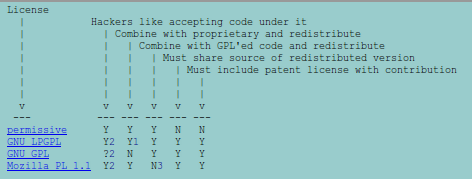
\includegraphics[width=11.5cm]{figs/licenses_quick_reference.png}
\end{center}

\end{frame}

%%%%%%%%%%%%%%%%%%%%%%%%%%%%%%%%%%%%%%%%%%%%%%%%%%%%%%%%%%%%%%%%%%%%%%%

\begin{frame}
\frametitle{Quick Reference For Choosing a Free Software License}

\begin{center}
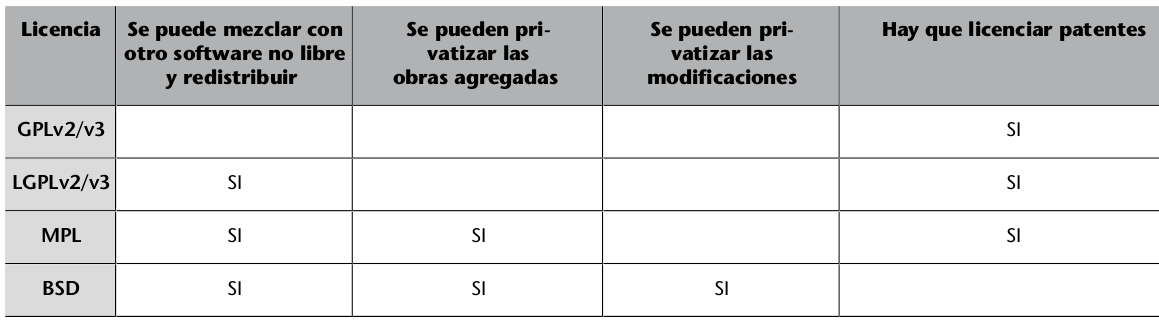
\includegraphics[width=11.5cm]{figs/tabla_licencias.png}
\end{center}

\end{frame}

%%%%%%%%%%%%%%%%%%%%%%%%%%%%%%%%%%%%%%%%%%%%%%%%%%%%%%%%%%%%%%%%%%%%%%%

\begin{frame}
\frametitle{Conventional Matrix}

\begin{center}
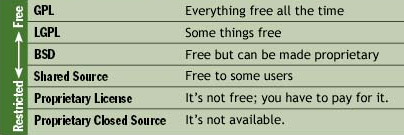
\includegraphics[width=11.5cm]{figs/conventional_matrix.png}
\end{center}

\end{frame}

%%%%%%%%%%%%%%%%%%%%%%%%%%%%%%%%%%%%%%%%%%%%%%%%%%%%%%%%%%%%%%%%%%%%%%%

\begin{frame}
\frametitle{Matrix Including Developer's Choice}

\begin{center}
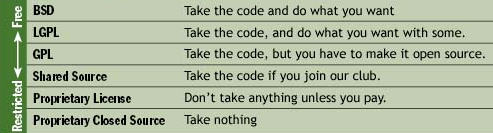
\includegraphics[width=11.5cm]{figs/matrix_developers_choice.png}
\end{center}

\end{frame}


%%%%%%%%%%%%%%%%%%%%%%%%%%%%%%%%%%%%%%%%%%%%%%%%%%%%%%%%%%%%%%%%%%%%%%%

\begin{frame}
\frametitle{Remarks}

\begin{itemize}
\item Some members of the community refuse to accept GPL'ed source code into their projects.
\item Other members of the community strongly prefer GPL'ed source code over other licenses.
\item Nobody refuses to accept code under permissive licenses such as BSD, X11, MIT... 
\end{itemize}

\end{frame}

%%%%%%%%%%%%%%%%%%%%%%%%%%%%%%%%%%%%%%%%%%%%%%%%%%%%%%%%%%%%%%%%%%%%%%%

\begin{frame}
\frametitle{Remarks (2)}

\begin{itemize}
\item Almost nobody refuses to accept LGPL'ed code, except the Apache Foundation, saying that they think it would impose LGPL requirement upon the proprietary code (when they are linked via the Java class-loading mechanism).
\item The FSF disagrees with this statement, asserting that such linking falls under section 6 of the LGPLv2 (linking exception).
\end{itemize}

\end{frame}

%%%%%%%%%%%%%%%%%%%%%%%%%%%%%%%%%%%%%%%%%%%%%%%%%%%%%%%%%%%%%%%%%%%%%%%

\begin{frame}
\frametitle{Remarks (and 3)}

\begin{itemize}
\item MPL 1.1 can be specifically amended to allow combining with GPL (section 13).
\item You should also get your employer (if you work as a programmer) or school, to sign a ``copyright disclaimer'' for the program, if necessary. 
\end{itemize}

\end{frame}


%%%%%%%%%%%%%%%%%%%%%%%%%%%%%%%%%%%%%%%%%%%%%%%%%%%%%%%%%%%%%%%%%%%%%%%

\begin{frame}
\frametitle{Applying a free license}


\begin{itemize}
\item \texttt{LICENSE} or \texttt{COPYING} file.
\item Copyright and license summary at the beginning of each source file.
\item It should have at least the ``copyright'' notice and a link to the full version of the license.
\item Also add information on how to contact you by electronic and paper mail.
\item If the program is interactive (terminal), make it output a short copyright notice 
when it starts in an interactive mode.
\item If it has a GUI, a menu can include copyright notice (or even the full license).
\end{itemize}

\end{frame}

%%%%%%%%%%%%%%%%%%%%%%%%%%%%%%%%%%%%%%%%%%%%%%%%%%%%%%%%%%%%%%%%%%%%%%%

\begin{frame}
\frametitle{Example: How to Apply the GPL to Your Work}

\footnotesize

\texttt{<one line with program's name and a brief idea of what it does.>} \\
\texttt{Copyright (C) <year>  <name of author>}

\medskip

\texttt{This program is free software: you can redistribute it and/or modify
    it under the terms of the GNU General Public License as published by
    the Free Software Foundation, either version 3 of the License, or
    (at your option) any later version.}

\medskip

\texttt{This program is distributed in the hope that it will be useful,
    but WITHOUT ANY WARRANTY; without even the implied warranty of
    MERCHANTABILITY or FITNESS FOR A PARTICULAR PURPOSE.  See the
    GNU General Public License for more details.}

\medskip

\texttt{You should have received a copy of the GNU General Public License
    along with this program.  If not, see <http://www.gnu.org/licenses/>.}


\end{frame}

%%%%%%%%%%%%%%%%%%%%%%%%%%%%%%%%%%%%%%%%%%%%%%%%%%%%%%%%%%%%%%%%%%%%%%%

\begin{frame}
\frametitle{Example: How to Apply the Apache License to Your Work}

\footnotesize

\texttt{Copyright [yyyy] [name of copyright owner]}

\medskip

\texttt{Licensed under the Apache License, Version 2.0 (the ``License'');
   you may not use this file except in compliance with the License.
   You may obtain a copy of the License at http://www.apache.org/licenses/LICENSE-2.0}

\medskip

\texttt{Unless required by applicable law or agreed to in writing, software
   distributed under the License is distributed on an ``AS IS'' BASIS,
   WITHOUT WARRANTIES OR CONDITIONS OF ANY KIND, either express or implied.
   See the License for the specific language governing permissions and
   limitations under the License.}


\end{frame}



%%%%%%%%%%%%%%%%%%%%%%%%%%%%%%%%%%%%%%%%%%%%%%%%%%%%%%%%%%%%%%%%%%%%%%%
\begin{frame}
\frametitle{Dual-licensing}

Distribute software under two different sets of terms and conditions. Motivations:

\begin{itemize}
\item License compatibility (Perl, Mozilla/Firefox, MySQL).
\item Market segregation based business models (MySQL Enterprise)
\item Allows the holder to offer customisations, early releases, generate other derivative works or grant rights to third parties to redistribute proprietary versions.
\end{itemize}

                                                 
\end{frame}


%%%%%%%%%%%%%%%%%%%%%%%%%%%%%%%%%%%%%%%%%%%%%%%%%%%%%%%%%%%%%%%%%%%%%%%

\begin{frame}
\frametitle{Compatibility}

\begin{itemize}
\item Two licenses are incompatible if it is not possible combining both works in compliance with the terms of  both licenses at the same time. 
\item It affects to distribution, not the use. 
\item If two licenses are free does, it doesn't imply are compatible. 
\item Copyleft licenses are mutually incompatible, unless compatibility is declared explicitly. 
\item Support for `` linking'': even if not allowed mix or integrate software with different licenses, maybe it can be linked. 
\end{itemize}

\end{frame}

%%%%%%%%%%%%%%%%%%%%%%%%%%%%%%%%%%%%%%%%%%%%%%%%%%%%%%%%%%%%%%%%%%%%%%%

\begin{frame}
\frametitle{Forking (1)}

\begin{itemize}
\item A piece of software is modified and developed separately by another team development, and distributed under a different name, and maybe other
license.
\item The forks can be possible \alert{only} with free/open source software.
\item The GPL software has tendency to avoid forking (we must keep the original license).
\item The BSD-style licenses are forked easily.
\end{itemize}

\end{frame}

%%%%%%%%%%%%%%%%%%%%%%%%%%%%%%%%%%%%%%%%%%%%%%%%%%%%%%%%%%%%%%%%%%%%%%%

\begin{frame}
\frametitle{Forking (and 2)}

\begin{itemize}
\item Forking is considered a bad thing (waste efforts, bitter disputes...).
\item But there are successful cases: XOrg/XFree86, 386BSD, OpenBSD, Gnu-Emacs/XEmacs, changes of license (GForge, OpenSSH).
\end{itemize}

\end{frame}


%%%%%%%%%%%%%%%%%%%%%%%%%%%%%%%%%%%%%%%%%%%%%%%%%%%%%%%%%%%%%%%%%%%%%%%

\begin{frame}
\frametitle{Licenses and warranty}

\begin{itemize}
\item Warranty disclaimers and limitation of liability clauses are common in software.
\item There are legal doubts about the effectiveness of these clauses: \alert{would not apply to consumers}.
\item This clauses are valid when there is \alert{no commercial service}.
\item The proprietary licenses using similar terms: is a myth to accept greater responsibility.
\item It must be considered legal guarantees that apply to both open source and proprietary software.
\item The free licenses allow (sometimes) to add extra warranty clauses.
\end{itemize}


\end{frame}

%%%%%%%%%%%%%%%%%%%%%%%%%%%%%%%%%%%%%%%%%%%%%%%%%%%%%%%%%%%%%%%%%%%%%%%

\begin{frame}
\frametitle{Exercise: Case study}


\begin{itemize}
\item Case study: Apache License v2 and GPL (v2 and v3)  (in)compatibility.
\end{itemize}

\end{frame}


%%%%%%%%%%%%%%%%%%%%%%%%%%%%%%%%%%%%%%%%%%%%%%%%%%%%%%%%%%%%%%%%%%%%%%%

\begin{frame}
\frametitle{Exercise: Case study}


\begin{itemize}
\item Case study: GPL and CDDL incompatibility.
\end{itemize}

\end{frame}

%%%%%%%%%%%%%%%%%%%%%%%%%%%%%%%%%%%%%%%%%%%%%%%%%%%%%%%%%%%%%%%%%%%%%%%

\begin{frame}
\frametitle{Case study: Apache License v2 and GPLv2 incompatibility}


\begin{itemize}
\item Apache License’s patent-licensing provision: each Apache contributor grants a user a license to use any patented software that falls under the license 
\item In exchange, the user agrees not to institute any patent-related litigation. 
\item The Apache License terminates upon any violation of this restriction. The GPLv2, which has a similar provision, does not.
\item This small difference led the FSF to declare the Apache License ``incompatible'' with the GPLv2: one of the fundamental tenets of the GPLv2 is that software distributed under it cannot be encumbered with further restrictions. 
\item What this controversy shows is that, sometimes, software developers need to think like lawyers when they use the different open source licenses. 
\end{itemize}

\end{frame}

%%%%%%%%%%%%%%%%%%%%%%%%%%%%%%%%%%%%%%%%%%%%%%%%%%%%%%%%%%%%%%%%%%%%%%%

\begin{frame}
\frametitle{Case study: Apache License v2 and GPLv3 Compatibility}


\begin{itemize}
\item GPLv3 license accepts Apache software into GPLv3 works (under GPLv3!).
\item However, GPLv3 software cannot be included in Apache projects. 
\item The licenses are incompatible in \alert{one direction} only. 
\item Apache software would have to be distributed under GPLv3.
\end{itemize}

\url{http://www.apache.org/licenses/GPL-compatibility.html}

\end{frame}


%%%%%%%%%%%%%%%%%%%%%%%%%%%%%%%%%%%%%%%%%%%%%%%%%%%%%%%%%%%%%%%%%%%%%%%

\begin{frame}
\frametitle{Clarifying GPL / CDDL Incompatibility}

CDDL-licensed code cannot be redistributed under any license that imposes restrictions that are not present in CDDL:

\begin{block}{CDDL, section 3.4 ``Application of Additional Terms''}
\footnotesize
You may not offer or impose any terms on any Source Code version that alters or restricts the applicable version of this License or the recipients' rights hereunder. 
\end{block}

The ``rights hereunder''(*) include the right granted to recipients to link CDDL ``Covered Code'' with private non-MPL code to form a ``Larger Work'' (CDDL sect. 3.6 ``Larger Works''). GPL does not give recipients any such right. Therefore, the recipient cannot change the licensing terms to apply the GPL instead of CDDL. 

\medskip

\footnotesize{(*) \textit{Hereunder:} ``Under or below this; subsequent to this.''}

\end{frame}


%%%%%%%%%%%%%%%%%%%%%%%%%%%%%%%%%%%%%%%%%%%%%%%%%%%%%%%%%%%%%%%%%%%%%%%

\begin{frame}
\frametitle{Clarifying GPL / CDDL Incompatibility}

GPL-licensed code cannot be redistributed under any license that imposes restrictions that are not present in GPL, or that does not support rights granted in GPL: 

\begin{block}{GPLv2, section 6}
\footnotesize
Each time you redistribute the Program (or any work based on the Program), the recipient automatically receives a license from the original licensor to copy, distribute or modify the Program subject to these terms and conditions. You may not impose any further restrictions on the recipients' exercise of the rights granted herein. 
\end{block}

\end{frame}

%%%%%%%%%%%%%%%%%%%%%%%%%%%%%%%%%%%%%%%%%%%%%%%%%%%%%%%%%%%%%%%%%%%%%%%

\begin{frame}
\frametitle{Clarifying GPL / CDDL Incompatibility}

CDDL permits recipients to subvert the fundamental GPL right ``to copy, distribute or modify the Program''. In addition to allowing linkage with proprietary code, CDDL permits the recipient to relicense binaries:

\begin{block}{CDDL, section 3.5. ``Distribution of Executable Versions''}
\footnotesize
You may distribute the Executable form of the Covered Software under the terms of this License or under the terms of a license of Your choice, which may contain terms different from this License, provided that You are in compliance with the terms of this License and that the license for the Executable form does not attempt to limit or alter the recipient's rights in the Source Code form from the rights set forth in this License.
\end{block}

\end{frame}

%%%%%%%%%%%%%%%%%%%%%%%%%%%%%%%%%%%%%%%%%%%%%%%%%%%%%%%%%%%%%%%%%%%%%%%

\begin{frame}
\frametitle{Clarifying GPL / CDDL Incompatibility}

This section (3.5), in turn, fails to satisfy the requirements of GPL, which states:

\begin{block}{GPLv2, section 3}
\footnotesize
The source code for a work means the preferred form of the work for making modifications to it. For an executable work, complete source code means all the source code for all modules it contains, plus any associated interface definition files, plus the scripts used to control compilation and installation of the executable. 
\end{block}

CDDL only requires that the source code to the covered code (including any modifications to the covered code) be made available, which is not sufficient to ensure that the recipient can actually modify a real program. 

\end{frame}




%%%%%%%%%%%%%%%%%%%%%%%%%%%%%%%%%%%%%%%%%%%%%%%%%%%%%%%%%%%%%%%%%%%%%%%

\begin{frame}
\frametitle{Clarifying GPL / CDDL Incompatibility}

The GPL license applies to entire works. When you modify a work by adding code, the additional code becomes part of the work (although only when it is distributed as part of the work), and as such must continue to be GPL-licensed: 

\begin{block}{GPLv2, section 2}
\footnotesize
These requirements apply to the modified work as a whole. If identifiable sections of that work are not derived from the Program, and can be reasonably considered independent and separate works in themselves, then this License, and its terms, do not apply to those sections when you distribute them as separate works. But when you distribute the same sections as part of a whole which is a work based on the Program, the distribution of the whole must be on the terms of this License, whose permissions for other licensees extend to the entire whole, and thus to each and every part regardless of who wrote it. \end{block}

\end{frame}



%%%%%%%%%%%%%%%%%%%%%%%%%%%%%%%%%%%%%%%%%%%%%%%%%%%%%%%%%%%%%%%%%%%%%%%
%%%%%%%%%%%%%%%%%%%%%%%%%%%%%%%%%%%%%%%%%%%%%%%%%%%%%%%%%%%%%%%%%%%%%%%

\begin{frame}
\frametitle{Clarifying GPL / CDDL Incompatibility}

The GPL states:
\begin{block}{GPLv2, section 2}
\footnotesize
If identifiable sections of that work are not derived from the Program, and can be reasonably considered independent and separate works in themselves, then this License, and its terms, do not apply to those sections when you distribute them as separate works. But when you distribute the same sections as part of a whole which is a work based on the Program, the distribution of the whole must be on the terms of this License, whose permissions for other licensees extend to the entire whole, and thus to each and every part regardless of who wrote it.
\end{block}

However, the CDDL states:
\begin{block}{CDDL, section 3.4}
\footnotesize
You may not offer or impose any terms on any Covered Software in Source Code form that alters or restricts the applicable version of this License or the recipients' rights hereunder.
\end{block}

\end{frame}

%%%%%%%%%%%%%%%%%%%%%%%%%%%%%%%%%%%%%%%%%%%%%%%%%%%%%%%%%%%%%%%%%%%%%%%

\begin{frame}
\frametitle{Clarifying GPL / CDDL Incompatibility}

One of these ``recipients' rights'' is:
\begin{block}{CDDL, section 3.6}
\footnotesize
You may create a Larger Work by combining Covered Software with other code not governed by the terms of this License and distribute the Larger Work as a single product. In such a case, You must make sure the requirements of this License are fulfilled for the Covered Software.
\end{block}

But the GPL terms forbids the user to combine any part of software with (for example) closed source software, thereby ``restricting the recipients' rights'' and meaning that the CDDL terms of the included module have not been followed.

\end{frame}

%%%%%%%%%%%%%%%%%%%%%%%%%%%%%%%%%%%%%%%%%%%%%%%%%%%%%%%%%%%%%%%%%%%%%%%

\begin{frame}
\frametitle{GPL / CDDL Incompatibility: Conclusions}

\begin{itemize}
\item A software containing a part CDDLed code and a part GPLed couldn't be legally delivered.
\item This incompatibility is not immediately obvious.
\item About MPL and GPL incompatibility issues: \url{http://www.tomhull.com/ocston/docs/mozgpl.html}
\end{itemize}

\begin{block}{The FSF states about CDDL:}
This is a free software license. It has a copyleft with a scope that's similar to the one in the Mozilla Public License, which makes it incompatible with the GNU GPL. This means a module covered by the GPL and a module covered by the CDDL cannot legally be linked together.
\end{block}

\end{frame}




%%%%%%%%%%%%%%%%%%%%%%%%%%%%%%%%%%%%%%%%%%%%%%%%%%%%%%%%%%%%%%%%%%%%%%%

\begin{frame}
\frametitle{Case study: The EUPL}


\begin{itemize}
\item Moodle Exercise 
\end{itemize}

\end{frame}

%%%%%%%%%%%%%%%%%%%%%%%%%%%%%%%%%%%%%%%%%%%%%%%%%%%%%%%%%%%%%%%%%%%%%%%

\begin{frame}
\frametitle{Case study: Protecting Users From Anti-Circumvention Law}

\pause

\small
``\textit{When you convey a covered work, you waive any legal power to forbid circumvention of technological measures to the extent such circumvention is effected by exercising rights under this License with respect to the covered work, and you disclaim any intention to limit operation or modification of the work as a means of enforcing, against the work's users, your or third parties' legal rights to forbid circumvention of technological measures..}'' (GPLv3, sect. 3)


\end{frame}

%%%%%%%%%%%%%%%%%%%%%%%%%%%%%%%%%%%%%%%%%%%%%%%%%%%%%%%%%%%%%%%%%%%%%%%

\begin{frame}
\frametitle{Case study: linking exception}

\pause

``\textit{As a special exception, the copyright holders of this library give you permission to link this library with independent modules to produce an executable, regardless of the license terms of these independent modules, and to copy and distribute the resulting executable under terms of your choice.}'' (GNU Classpath)

\end{frame}


%%%%%%%%%%%%%%%%%%%%%%%%%%%%%%%%%%%%%%%%%%%%%%%%%%%%%%%%%%%%%%%%%%%%%%%

\begin{frame}

\begin{center}
\huge{Legal Myths}
\end{center}

\end{frame}


%%%%%%%%%%%%%%%%%%%%%%%%%%%%%%%%%%%%%%%%%%%%%%%%%%%%%%%%%%%%%%%%%%%%%%%

\begin{frame}

\begin{center}
\huge{``Free software hasn't owners or copyright holders''}
\end{center}

\end{frame}

%%%%%%%%%%%%%%%%%%%%%%%%%%%%%%%%%%%%%%%%%%%%%%%%%%%%%%%%%%%%%%%%%%%%%%%

\begin{frame}

\begin{center}
\huge{``The free licenses force to grant copyrights.''}
\end{center}

\end{frame}


%%%%%%%%%%%%%%%%%%%%%%%%%%%%%%%%%%%%%%%%%%%%%%%%%%%%%%%%%%%%%%%%%%%%%%%

\begin{frame}

\begin{center}
\huge{``Free software and proprietary software are incompatible''}
\end{center}

\end{frame}


%%%%%%%%%%%%%%%%%%%%%%%%%%%%%%%%%%%%%%%%%%%%%%%%%%%%%%%%%%%%%%%%%%%%%%%

\begin{frame}

\begin{center}
\huge{``It's not possible merge open source and proprietary software.''}
\end{center}

\end{frame}


%%%%%%%%%%%%%%%%%%%%%%%%%%%%%%%%%%%%%%%%%%%%%%%%%%%%%%%%%%%%%%%%%%%%%%%

\begin{frame}

\begin{center}
\huge{``Copyleft licenses force to publish derivate works.''}
\end{center}

\end{frame}


%%%%%%%%%%%%%%%%%%%%%%%%%%%%%%%%%%%%%%%%%%%%%%%%%%%%%%%%%%%%%%%%%%%%%%%

\begin{frame}

\begin{center}
\huge{``Free software don't have neither warranties nor liability.''}
\end{center}

\end{frame}


%%%%%%%%%%%%%%%%%%%%%%%%%%%%%%%%%%%%%%%%%%%%%%%%%%%%%%%%%%%%%%%%%%%%%%%

\begin{frame}

\begin{center}
\huge{``The diversity of free licenses is positive.''}
\end{center}

\end{frame}


%%==================================================================
%%---------------------------------------------------------------


